
\documentclass[12pt]{article}
\usepackage[margin=1in]{geometry}
\usepackage[pdftex]{graphicx}
\usepackage{multirow}
\usepackage{setspace}
\usepackage{enumitem}
\pagestyle{plain}
\setlength\parindent{0pt}

\begin{document}

% Course information
\begin{tabular*}{\textwidth}{l @{\extracolsep{\fill}} r}
  & \multirow{3}{*}{
\includegraphics[height=1.0in]{logo.jpg}} \\
  \large 116C Title & \\
  \large Spring Quarter 2018 & \\
  \large Physics 116C & \\
\end{tabular*}
\vspace{10mm}

% Professor information
\begin{tabular}{ l l }
  \multirow{6}{*}{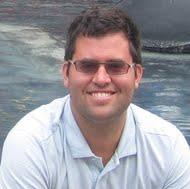
\includegraphics[height=1.25in]{mike.jpg}} & \\
  & \\
  & \large Michael Mulhearn \\
  & \large mulhearn@physics.ucdavis.edu \\
  & \large Physics 317 \\
  & \\
\end{tabular}
\vskip 0.5cm
\noindent
\textbf {Lectures:} M,W,F 12:10-1:00 PM in Rm. 140 Physics
\begin{tabbing}
\hspace*{3em}\= \hspace*{5em} \= \kill % set the tabbings
\textbf {Lab:}    \> Section 1: \>  M 3:10-6:00 PM in Rm. 152 Roessler \\
                        \> Section 2: \> W 3:10-6:00 PM in Rm. 152 Roessler \\
\end{tabbing}

\noindent
\textbf {Texts:} \emph{The Art of Electronics}, 3\textsuperscript{rd} Edition, Horowitz and Hill\\
{\tt https://www.scipy-lectures.org/\_downloads/ScipyLectures-simple.pdf} \\
\noindent
\textbf{Office Hours:} W 2:00-3:00 PM in 152 Roessler, and also often available during lab.\\
\noindent
\textbf{Lab Instructor:} Christopher Brainerd, cbbrainerd@ucdavis.edu \\
\noindent
\textbf{Midterm Exams:} Two Midterm Exams,  TBA \\ 
\textbf{Final Exam:} Monday, December 11 at 3:30 pm \\
\textbf{Homework:}  There will be approximately five homework assignments.\\

\noindent
\textbf {Course Description:}  This course covers analog electronic devices from passive components resistors, capacitors, and inductors to active devices diodes, transistors, and operational amplifiers.   It includes physical models for analog devices, circuit design and analysis, and laboratory techniques. \\

\noindent
\textbf {Course Objections:} 
You will gain  lab experience with measurement and debugging of analog electric circuits.  You will learn practical mathematical tools for analyzing or designing and tuning circuits.  You will apply basic physics principles toward understanding realistic models for the response of passive and active electronic components. \\

\noindent
\textbf {Lab Safety:} 
You should complete the online course for Electrical Safety at \\
{\tt http://safetyservices.ucdavis.edu/training/electrical-safety}.\\

\noindent
\textbf {Lab Reports:} 
Before each lab, download the lab write-out, print it out, and complete the pre-lab computations. Online logs are very useful, but a hand-written logbook is still hard to beat. For this class, bring a quadrille-ruled notebook for lab notes and quick hand-written plots, which you may supplement with an online logbook if you prefer. Note that if you use an online tool, you'll still need to provide a collated paper log to your TA. Data sheets can be shared via photo-copying or online logs, but each student must maintain their own log.  Students should also bring a flash drive to transfer scope images to a laptop for preparation of lab reports.
The TA will provide more information.


\vskip 0.5cm
\noindent
\textbf {Tentative Course Outline}:

The weekly coverage might change as it depends on the progress of the class.    Most weeks we'll need to cover some additional material to prepare for the upcoming labs.



\begin{table}[h!]
\normalsize % The size of the table text can be changed depending on content. Remove if desired.
\begin{tabular}{ llll }
\hline
\textbf{Week} & \textbf{Dates} & \textbf{Lecture} & \textbf{Lab} \\
\hline
1 & 2,4,6 Apr & Microprocessors and Assembly & 1) Intro to Arduino and Scipy \\
\hline
2 & 9,11,13 Apr &  & 2) Arduino Digital Scope \\
\hline
3 & 16,18,20 Apr & Statistical Distributions & 2) Arduino Digital Scope  \\
\hline
4 & 16,18,20 Apr & Uncertainties & 3) Geiger Counter \\
\hline
5 & 23,25,27 Apr & Fourier Transform& 3) Geiger Counter \\
\hline
6 & 30 Apr 2,4 May & Noise & 4) Fast Fourier Transform \\
\hline
7 & 7,9,11 May & Statistical Analysis & 5) Johnson Noise \\
\hline
8 & 14,16,18 May &  & 5) Johnson Noise \\
\hline
9 & 21,23,25 May & & 6) PID Controller\\
\hline
10 & (28),30 May,1 Jun & &  No Lab \\
\hline
11 &  4,6 Jun &  & 7)  Arithmetic Logic Unit\\
\hline
\end{tabular} 
\end{table}

\end{document}

